This chapter lists the requirements for the effects presented in the analysis. 

\begin{figure}[htbp]
	\centering
\begin{picture}(0,0)%
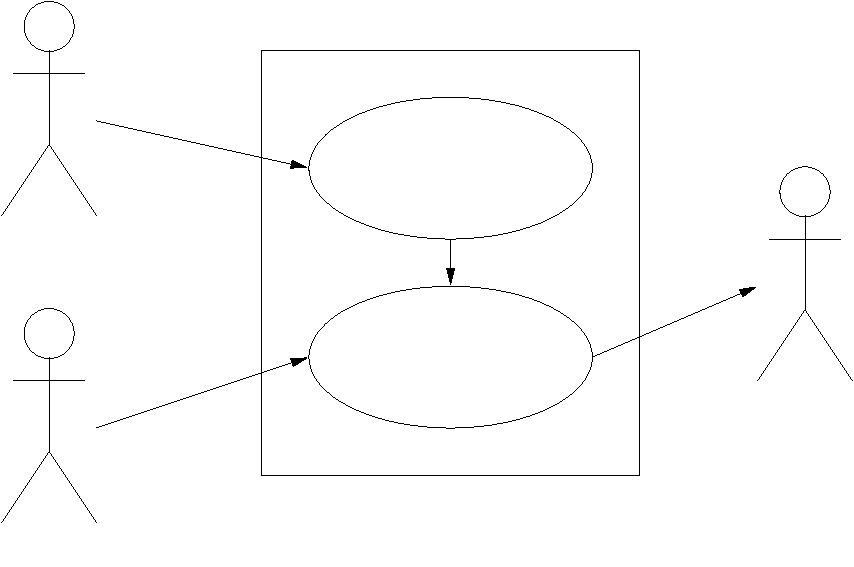
\includegraphics{Use_case.pdf}%
\end{picture}%
\setlength{\unitlength}{4144sp}%
%
\begingroup\makeatletter\ifx\SetFigFont\undefined%
\gdef\SetFigFont#1#2#3#4#5{%
  \reset@font\fontsize{#1}{#2pt}%
  \fontfamily{#3}\fontseries{#4}\fontshape{#5}%
  \selectfont}%
\fi\endgroup%
\begin{picture}(6507,4318)(1426,-4900)
\put(1531,-2491){User}%
\put(4546,-3346){Effect}%
\put(4276,-1906){Effect select}%
\put(7111,-3751){Amplifier}%
\put(1441,-4831){Guitar}%
\end{picture}%
	\caption{A graphically overview of wanted functionality in form of an use case digram.}
	\label{fig:use_case}
\end{figure}

From \autoref{ch:analysing} some of the effect can be designed together, because the effect is using the same parts but multiply times or just a small difference. The following description tells shortly about the different in the effect block and which effect that can be designed together.

\paragraph*{Basic filtering}
The only basis filter, which is explained in \autoref{ch:analysing} which is a basic filter without delay and time changing parameters is the Equalizer.

\paragraph{Time varying filter}
The only Time varying filter, which is explained in \autoref{ch:analysing} is the Wah-Wah.

\paragraph{Delay}
All the delay based effect have at lest one delay block and have both fast and slow delay. All the analysed delayed based effect in \autoref{ch:analysing} is:
\begin{itemize}
	\item Delay
	\item \gls{reverb}
	\item Flanger
	\item Chorus
\end{itemize} 

The block diagram in each effect shows that pair wise effect have a common structure with using the same parts but multiply times. The chorus is the flanger with the same effect added more than once. The same is applicable by delay and \gls{reverb} respectively. Then the only two effect which needed to be designed is Chorus and \gls{reverb} because Flanger and Delay can easily be made out of removing the multiply parts in their respectively effect.

\paragraph{Non-linear processing}
\begin{itemize}
	\item Distortion
	\item Overdrive
\end{itemize} 

\subsection{Block}

The requirements are divided into units, based on the effect analysis \autoref{ch:analysing}, since it is concluded in \autoref{ch:analysing} that only six general units need to be designed and all the presented effects can be created with those six. The unit that are going to be designed are the:



\begin{itemize}
	\item Bandpass filter
	\item Inverse bandpass filter
	\item Delay
	\item Gain
	\item Clipping
	\item \gls{lfo}
\end{itemize} 

 Besides the fact that each unit shall be designed individually, each unit interface should fit in the effect that is using it. Each unit has its own section where the requirements and their arguments are presented. To ensure that the units can fit and work together, basic requirements  are made on the processing component to be chosen afterwards first.
 
 